\documentclass{article}
% -------- Umlaute korrekt ----------------
\usepackage[latin1, utf8]{inputenc}
\usepackage[ngerman]{babel}
\usepackage{graphicx}
%-------------------------------------------

% Einrueckung unterbinden nach Absatz
\setlength{\parindent}{0pt}

\DeclareMathSizes{10}{10}{10}{10}
\title{RA -- R\"U Blatt 1}
\author{Christian Bay (lu38wuqi), Tobias Miksch (up83yvev)}
\date{\today}
\begin{document}
\maketitle

\textbf{ICC Version:}
\begin{enumerate}
	\item intelmpi/4.1.3.048-intel
	\item mkl/11.0up05
	\item intel64/13.1up03
\end{enumerate}

\vspace*{6pt}

\section*{Aufgabe 3}
\subsection*{b)}

\begin{center}
	\begin{figure}[h]
	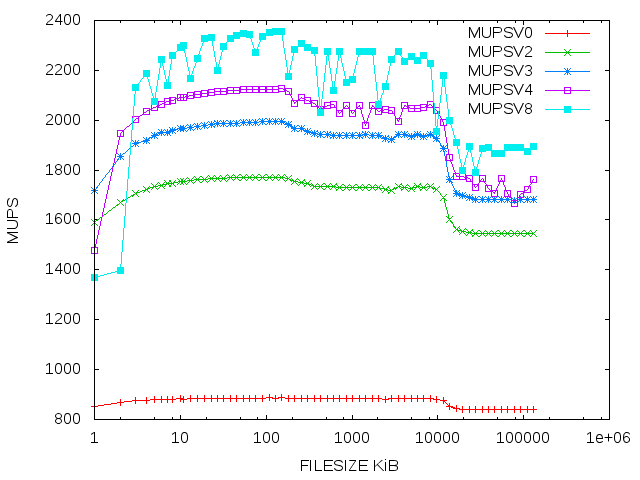
\includegraphics[scale=0.6]{pics/a3b.png}
	\caption{Plot of manual loop unrolling}
	\end{figure}
\end{center}

\subsection*{c)}
\begin{itemize}
	\item Geschwindigkeit steigt an bis 3 faches manuelles unrolling.
		Danach verhalten sich Werte sehr ähnlich
	\item \textbf{Ursache:} Taktdauer von ADDSS (3 Takte)
\end{itemize}

\section*{Aufgabe 4}
\subsection*{b)}

\begin{center}
	\begin{figure}[h]
	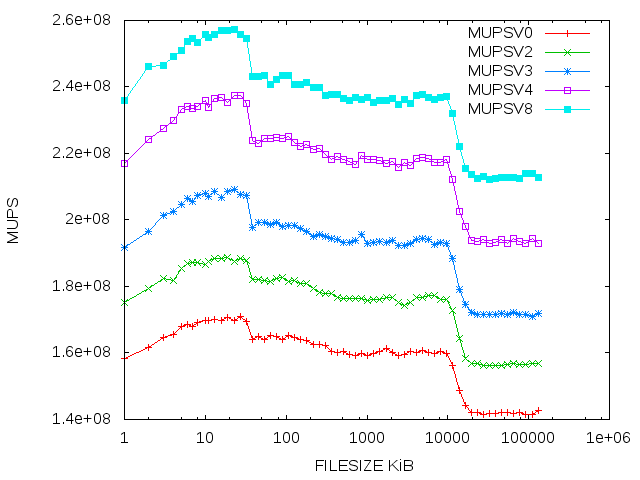
\includegraphics[scale=0.6]{pics/a4b.png}
	\caption{Plot of compiler based loop unrolling}
	\end{figure}
\end{center}

\subsection*{c)}
Cache Daten von Lima:\\
\begin{center}
	\begin{tabular}{| c || c |}
		\hline
		Cache-Typ             & Gr\"osse \\
		\hline
		\hline
		L1d cache             &    32K\\
		\hline
		L1i cache             &    32K\\
		\hline
		L2 cache              &    256K\\
		\hline
		L3 cache              &    12288K\\
		\hline
	\end{tabular}
\end{center}

\begin{itemize}
	\item Maximale Geschwindkeit tritt bei Vektorgr\"osse kleiner gleich $\approx 32$ KiB auf.
		\begin{enumerate}
			\item Geschwindigkeitsverlust ab $32$ KiB\\ \textbf{Ursache:} Cache L1D voll
			\item Geschwindigkeitsverlust ab $10.000$ KiB\\ \textbf{Ursache:} Cache L3 voll
		\end{enumerate}
\end{itemize}

\end{document}
